%%==================================================
%% chapter02.tex for SJTU Bachelor Thesis
%% version: 0.5.2
%% Encoding: UTF-8
%%==================================================

\chapter{模块化结构的设计与改良}
\label{chap:mechanicalSystem}
对于控制系统的设计,往往也会涉及到机械结构的配套设计。一个控制系统对于机器人控制的实现,是要通过执行器来实现的,因此控制器往往会对执行器的外观有一定的要求;同时控制器决策的确定,是需要传感器辅助来实现的,因此传感器对于所在的机器人本体也会有一定的要求。综上所述,机械结构的设计是控制系统设计的前提。在本章中,会给出和控制系统相关的机械结构的设计细节,以期起到对于后面的控制系统设计的辅助说明。

\section{先前设计方案的回顾}
<<<<<<< HEAD
本文所设计的控制系统是以所在实验室先前设计的太阳能驱动模块化机器人作为控制对象原形来进行设计的。所以在对本文所涉及的对于机械结构的改进与重设计之前,对前人的设计方案进行回顾是有必要的。原模块化机器人拼接成的太阳能机器人的3D模型和实物图如图\ref{fig.OriginalModel} 所示。 \\
=======
本文所设计的控制系统是以所在实验室先前设计的太阳能驱动模块化机器人作为控制对象原形来进行设计的。原模块化机器人拼接成的太阳能机器人的3D模型和实物图如图\ref{fig.OriginalModel} 所示。 \\
>>>>>>> 344532f7f0d9415fa34ed575a4c3b19c275e0e14
\begin{figure}
  \centering
  \subfigure[3D模型图]{
    \label{fig:corereal:a} %% label for first subfigure
    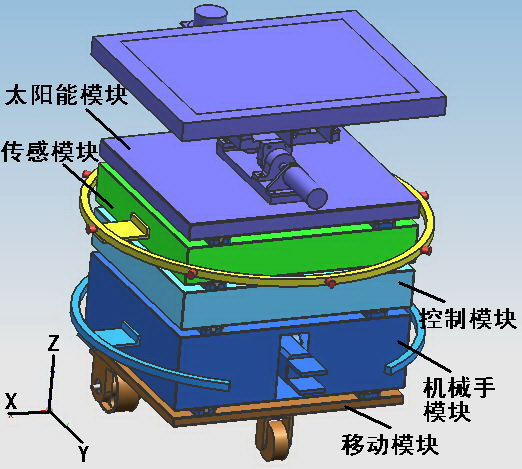
\includegraphics[width=0.35\textwidth]{chap2/Original3DModel.png}}
  \hspace{1in}
  \subfigure[实物图]{
    \label{fig:corereal:b} %% label for second subfigure
    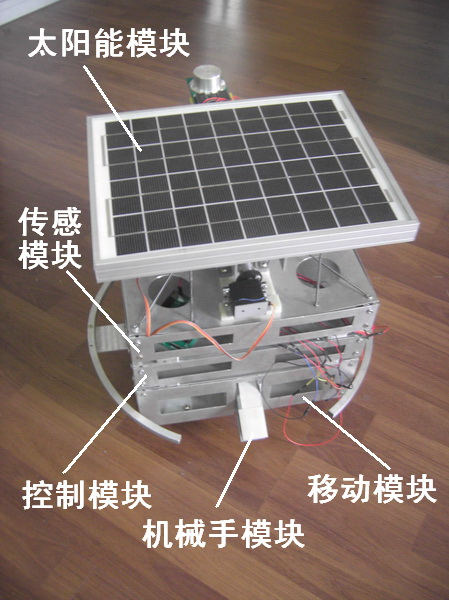
\includegraphics[width=0.35\textwidth]{chap2/OriginalRealModel.PNG}}
  \bicaption[fig.OriginalModel]{原设计方案模型}{原设计方案模型}{Fig}{The Model of the Original Design}
\end{figure}
原机器人的坐标系规定如下:

原点O取为移动模块两驱动轮中心连线的中点,Z轴垂直机器人底面向上,Y轴沿机器人前进方向,X轴由右手定则确定。太阳能驱动模块化机器人结构与坐标方向示意如图\ref{fig:corereal:a} 所示。
\subsection{传感器模块结构}
传感模块主体为立方壳体,模块上、下表面分别安装上、下接口。两侧分别固定一个支架,再在支架上固定一个圆环,在圆环的前、后、左、右及左前、右前、左后、右后的八等分圆处分别安装一个超声波传感器。主要用于实现对八个方位的障碍物探测与测距功能。如图\ref{fig.SensorSupport} 所示。
\begin{figure}[!htp]
  \centering
  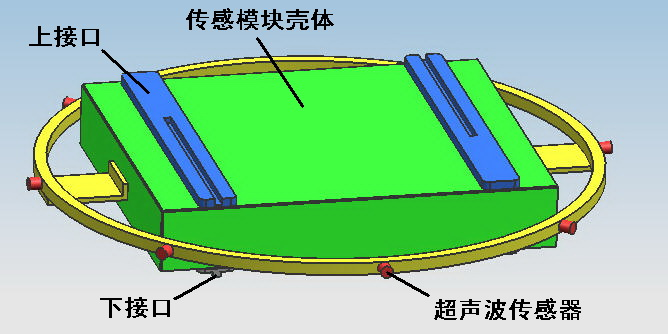
\includegraphics[width=0.8\textwidth]{chap2/OriginalSensorSupport.PNG}
  \bicaption[fig.SensorSupport]{原设计方案传感器支架}{原设计方案传感器支架}{Fig}{The Sensor Stand of Original Design}
\end{figure}
\subsection{控制模块结构}
控制模块主体也为立方壳体,模块上、下表面也分别安装上、下接口。其内安装主控制系统电路板和双轴陀螺仪、电子罗盘等,实现机器人自身的倾角和方位测量等功能,接收传感模块输入的障碍物探测信息,并输出对移动模块和机械手模块的控制信号。如图\ref{fig.CentralUnit} 所示。
\begin{figure}[!htp]
  \centering
  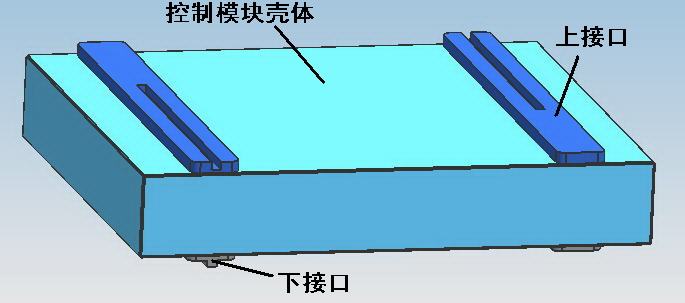
\includegraphics[width=0.8\textwidth]{chap2/OriginalCentralUnit.PNG}
  \bicaption[fig.CentralUnit]{原设计方案控制模块}{原设计方案控制模块}{Fig}{The Control Module of Original Design}
\end{figure}
\subsection{移动模块结构}
移动模块主体为较薄的立方壳体,模块上表面安装上接口,下表面安装两个驱动轮和一个从动脚轮。两个驱动轮分别由一个直流电机带动,利用两驱动轮差速运动实现转向运动;从动脚轮具有两个自由度,在摩擦作用下可以自动适应转动方向;磁珠装于轮轴上,通过安装于底盘上的霍尔传感器输出转速信息给控制模块。如图\ref{fig.ChesisOld} 所示。
\begin{figure}[!htp]
  \centering
  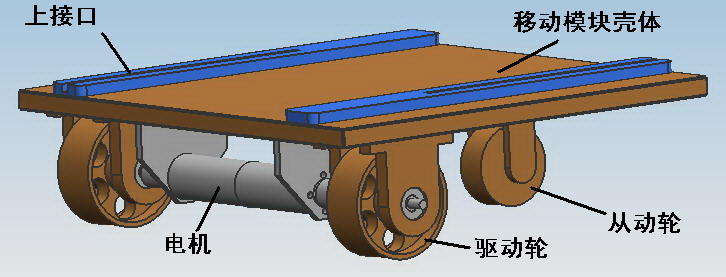
\includegraphics[width=0.8\textwidth]{chap2/OriginalChesis.PNG}
  \bicaption[fig.ChesisOld]{原设计方案移动模块}{原设计方案移动模块}{Fig}{The Mobile Module of Original Design}
\end{figure}
\subsection{标准化机电接口}
原方案设计的接口如图\ref{fig.OriginalPort} 所示。
\begin{figure}
  \centering
  \subfigure[下接口]{
    \label{fig:port:a} %% label for first subfigure
    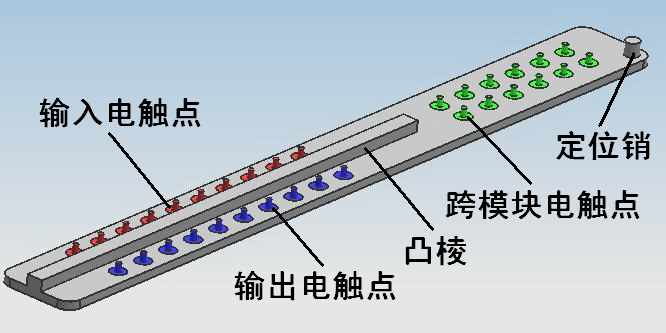
\includegraphics[width=0.4\textwidth]{chap2/OriginalPortUp.png}}
  %\hspace{1in}
  \subfigure[上接口]{
    \label{fig:port:b} %% label for second subfigure
    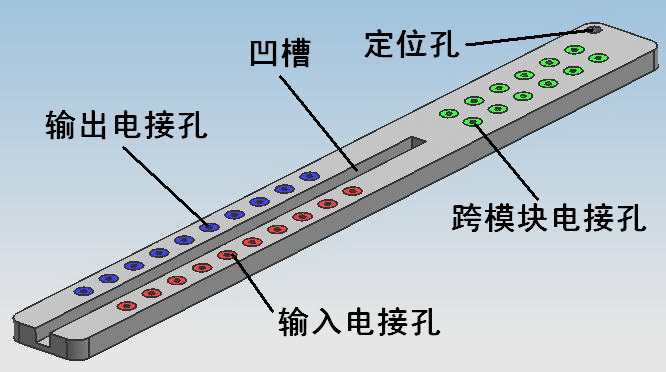
\includegraphics[width=0.4\textwidth]{chap2/OriginalPortDown.PNG}}
  \bicaption[fig.OriginalPort]{原设计方案标准化接口}{原设计方案标准化接口}{Fig}{The Communication Port Original Design}
\end{figure}
对接时,下接口面上的凸棱与上接口面上的凹槽配合,可限制对接的模块在X方向上的滑动自由度,再加上定位销与定位孔的配合,可限制模块沿着凹槽在Y方向上的滑动自由度,而上接口与下接口面配合,可限制垂直模块底面的Z方向上的平移自由度。如此,可方便地进行模块的机械对接。

\section{通用可扩展模块的补充设计}
在新的机器人系统中,将不再采用以前机器人的控制结构。在上面的介绍中,可以获知以前机器人拥有单一控制模块,所有其他模块都由这单一的模块进行控制。这就要求控制系统在新加入模块时要对总控制模块再编程。而且对于这种设计,为了实现其他模块的功能,不得不将大量的控制接口引出,集成在机械结构上,如上一节标准化机电接口设计所述。这种做法存在众多缺点。首先,接出来的众多接口提高了模块系统的复杂性,这些结构必须以有一定的形式存在于整合机器人个体的各个模块上,但是提供接口的上层模块却未必会用到接口功能,这就产生了设计资源与加工资源的浪费;其次这种设计缺少灵活性,在新加入功能模块或是主控芯片变动时,需要对接口进行再设计与加工,不利于机器人模块的升级使用;第三机械触点式接口易于磨损,长期使用的可靠性极差。综上所述,本设计提供了一种新的思路去解决上面所述的种种问题。

将对于模块的控制电路集成在各个模块上,即抛弃主控模块的概念,而在各个模块上设置控制电路,是每个模块可以脱离主体进行单独工作。这样只需要一种协调各模块的机制就可以了。现存的多种基于嵌入式系统的通讯机制可以满足这一要求。不过在众多系统中CAN总线系统及协议,是相对最好的解决方案,也是本设计所采用的方案。其有如下优点,第一,CAN总线接线简单,总线中只有CANH和CANL两条线;第二,协议成熟,这一协议的2.0版本是由博世公司于1996年提出的。至今经过了10余年的使用足以证明这个协议的可靠性;三,可靠性高,因为依赖的连线比较少,所以容错率会比SCI,SPI,$I^2C$等其他协议要高;四,可适用于大规模集群网络,就是指可以使众多模块在系统中协同工作。

根据这一思路,对系统进行了设计。关于电路硬件部分的详细说明请见下一章相应部分内容。在本节和下一节将给出根据此思想所设计的通用机械模块和模块间通讯接口的机械设计。

新的模块设计三维立体图如图\ref{fig.NewModuleBody} 所示,用于连接上下两个模块的槽型和凸起机构如图\ref{fig.SlotAndHeave} 所示。其中模块结构包括上下两个交叉的加强筋和一个电路板固定区,以及可以扩展的侧方空间。
\begin{figure}[!htp]
  \centering
  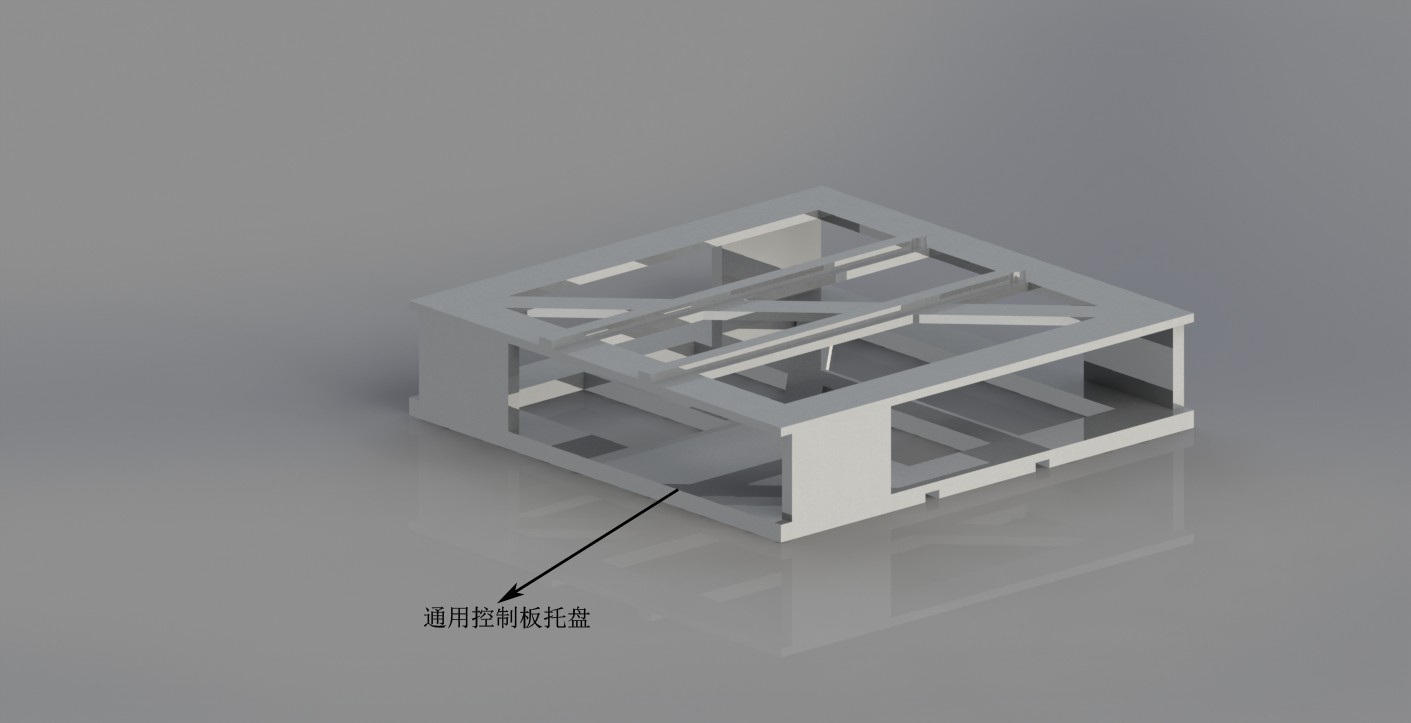
\includegraphics[width=0.8\textwidth]{chap2/NewModel.png}
  \bicaption[fig.NewModuleBody]{新设计的通用模块三维立体图}{新设计的通用模块三维立体图}{Fig}{The General Module of New Design}
\end{figure}
\begin{figure}
  \centering
  \subfigure[处于模块上端面的凸起]{
    \label{fig:cnt:a} %% label for first subfigure
    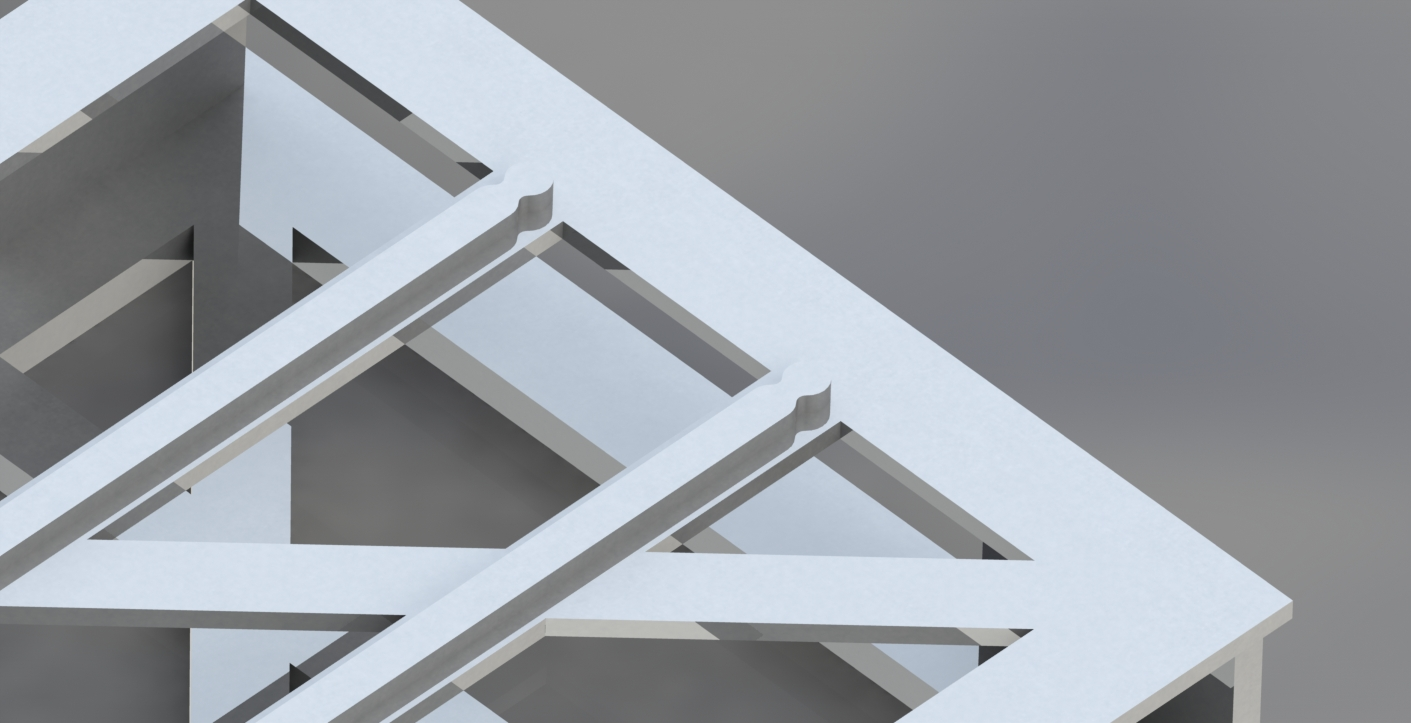
\includegraphics[width=0.4\textwidth]{chap2/LockHead.JPG}}
  %\hspace{1in}
  \subfigure[处于模块下端面的凹槽]{
    \label{fig:cnt:b} %% label for second subfigure
    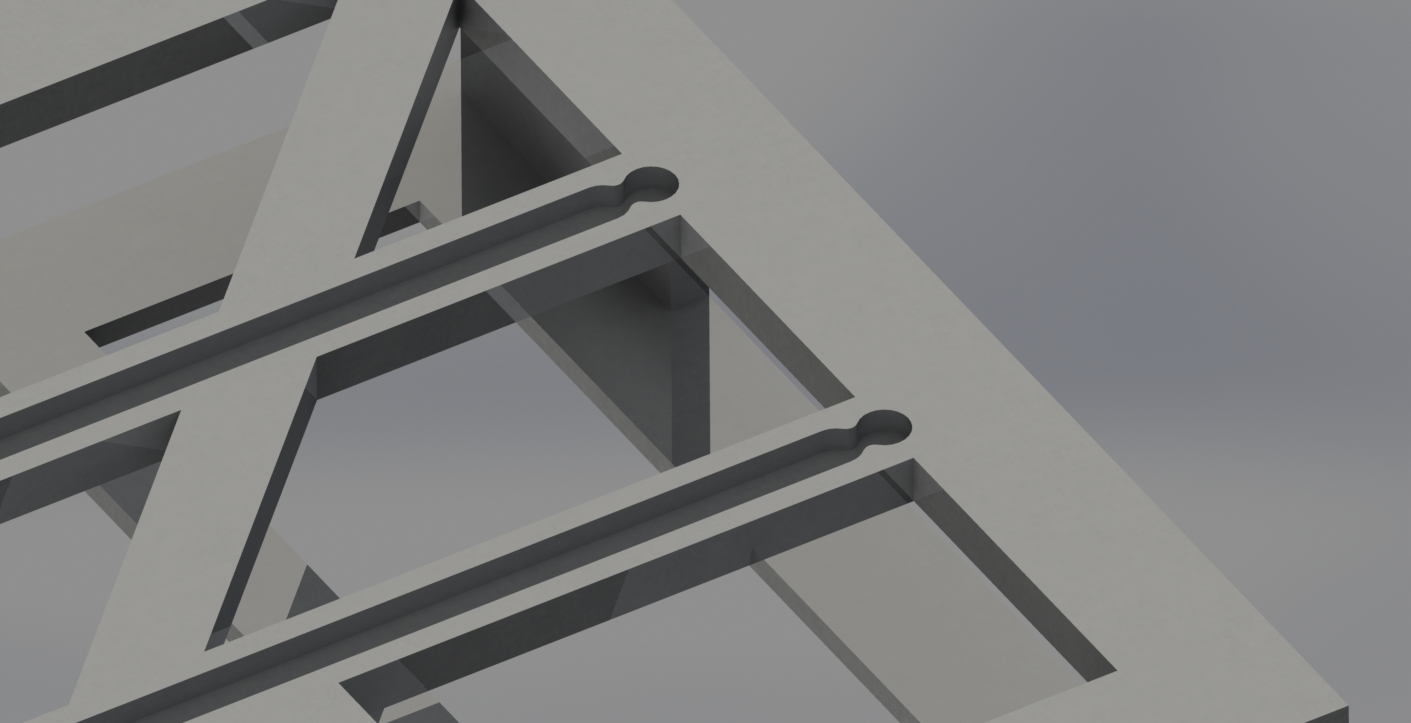
\includegraphics[width=0.4\textwidth]{chap2/LockSlot.JPG}}
  \bicaption[fig.SlotAndHeave]{新设计的通用模块的连接机构}{新设计的通用模块的连接机构}{Fig}{The Connection Structure of the New Design}
\end{figure}
\section{模块间通用接口的设计}
模块间通用接口既是固定在通用模块体上的,实现模块间通讯的接口电路板的机械固定装置。正如前文说明的那样,为了提高稳定性和简化模块结构,本设计决定使用CAN总线作为传输途径。但是又如前文分析的那样,如果采用接触式方案,将极易磨损而使传输变得不可靠。所以这里采用了光学手段,将总线中的高低电平变成红外LED的亮灭,而另一模块则通过一个光敏三极管接收传过来的光信号,并变回电信号传回另一模块的总线中去。因为光敏三极管是一个极其敏感的元件,为了避免不同光源之间的相互干扰,需要使对应的红外LED和光敏三极管处于同一个密封环境,这就需要在设计机械结构上得以实现。关于转换电路的内容会在第三章相应部分进行详细介绍。而接口的机械接口如图\ref{fig.ComuPort}所示,其位于槽和凸起的末端。
\begin{figure}
  \centering
  \subfigure[处于凸起上的接口]{
    \label{fig:Newport:a} %% label for first subfigure
    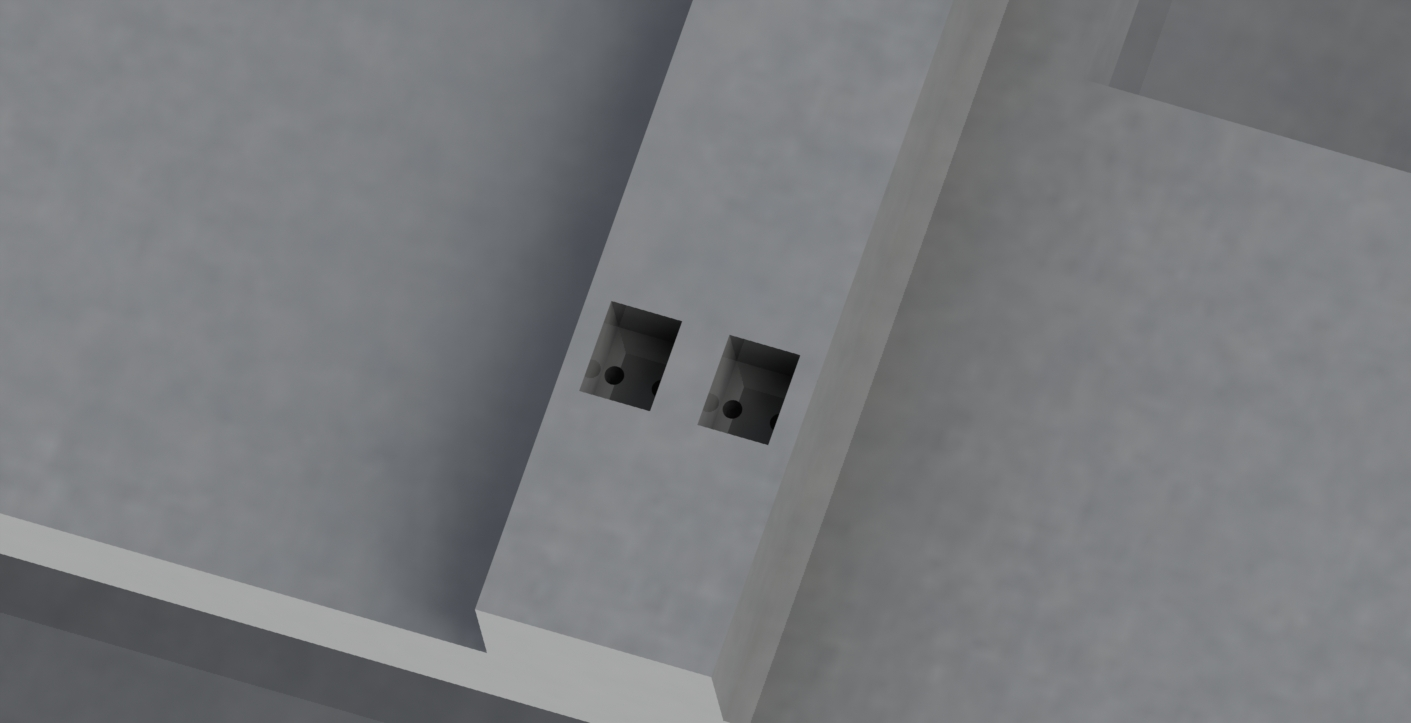
\includegraphics[width=0.4\textwidth]{chap2/PortOnHeave.JPG}}
  %\hspace{1in}
  \subfigure[处于凹槽上的接口]{
    \label{fig:Newport:b} %% label for second subfigure
    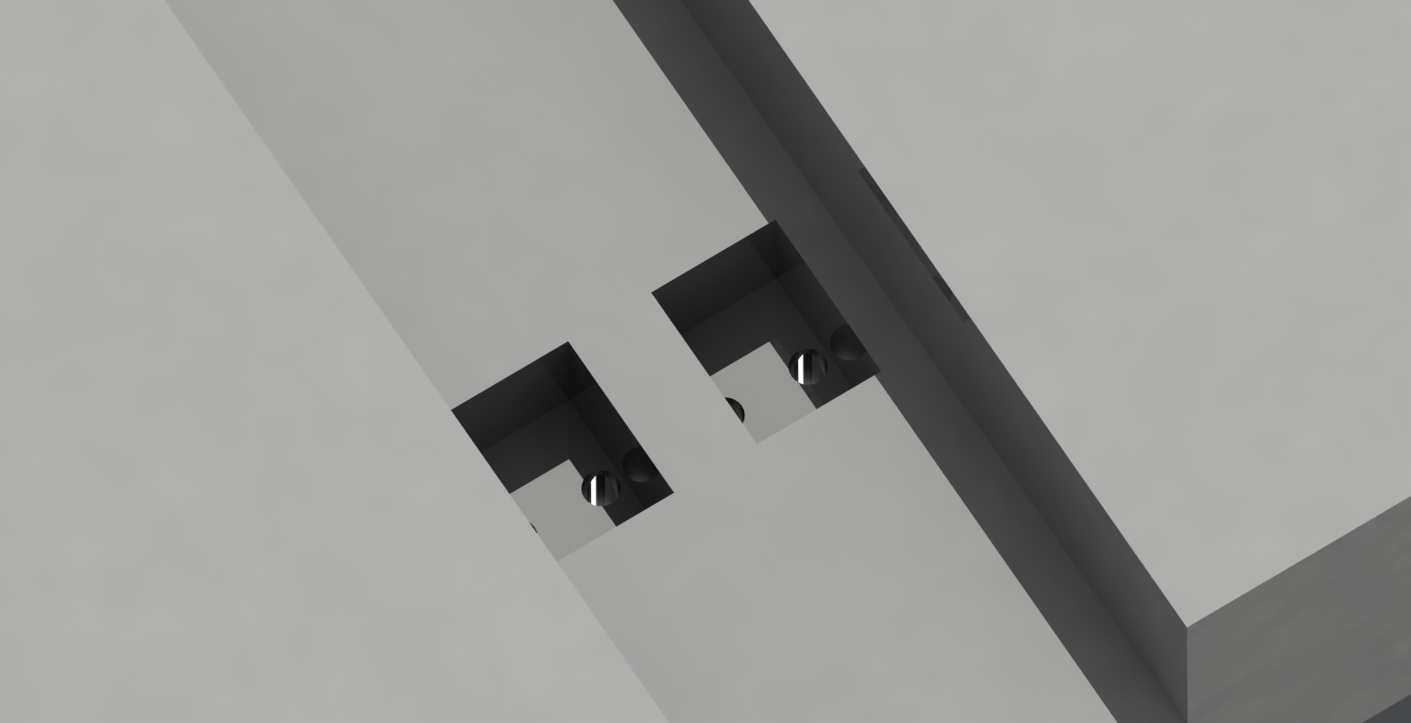
\includegraphics[width=0.4\textwidth]{chap2/PortOnSlot.JPG}}
  \bicaption[fig.ComuPort]{新设计的CAN总线接口}{新设计的CAN总线接口}{Fig}{The Communication Port of the New Design}
\end{figure}
\section{超声波传感器支架的设计}
因为定位的原因,本设计对传感器支架进行了重新设计。虽然圆形的传感器排布可以实现对环境的较好的检测,但是对于计算车体相对于障碍物的相对位置却变得非常复杂。为了解决这一问题,本设计重新对传感器的位置进行了安排。先前的设计文献中只把传感器作为圆柱处理,这显然是不现实的,在这里本设计对传感器尺寸进行了仔细测量,并按实际尺寸画出了传感器对于传感器支架的安装位置。其设计图如图所\ref{fig.NewSensorSupport}示。图中为传感器模块一侧传感器支架的样子,在模块的四个边上各有一个支架,每个支架上有三个超声波传感器。
\begin{figure}[!htp]
  \centering
  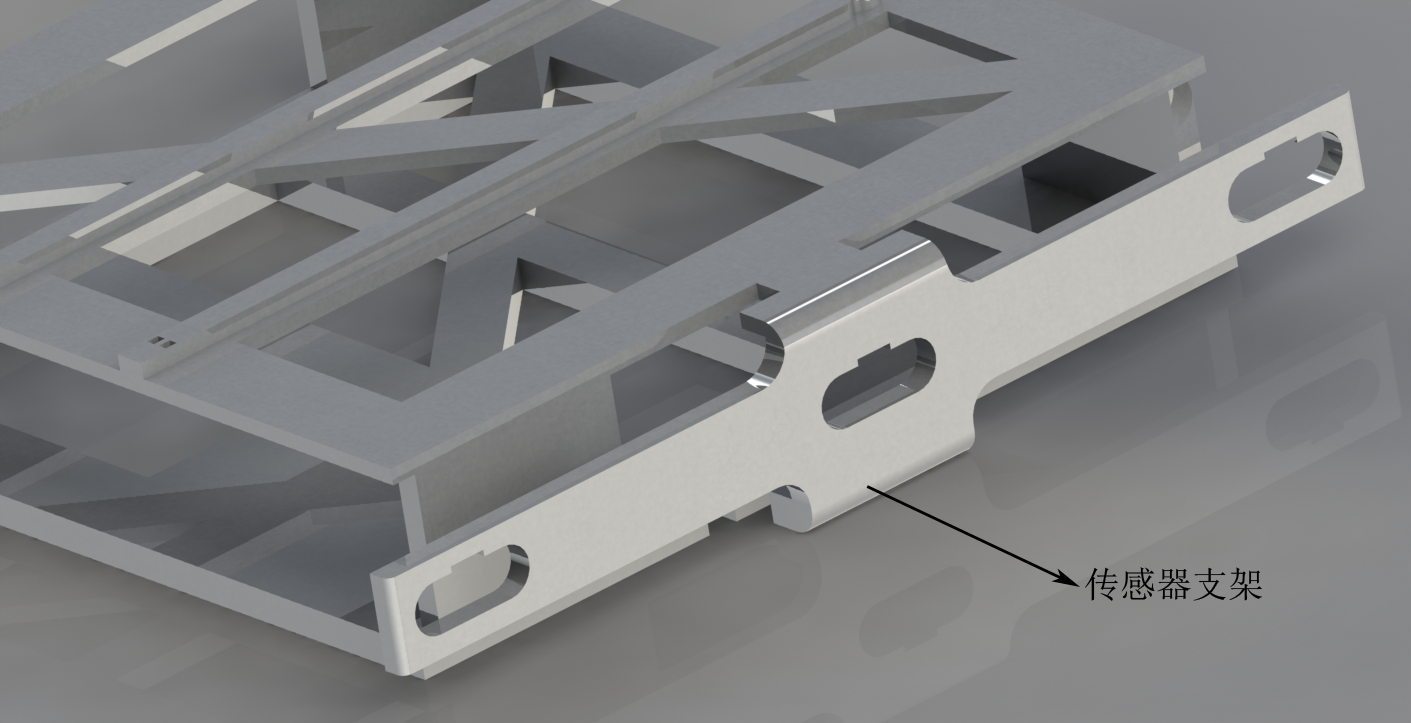
\includegraphics[width=0.8\textwidth]{chap2/SensorSupport.png}
  \bicaption[fig.NewSensorSupport]{新设计的传感器支架三维立体图}{新设计的传感器支架三维立体图}{Fig}{The General Module of Sensor Stand}
\end{figure}
\section{底盘编码轮的设计}
最直观的的对于二维坐标的测量莫过于直接测量车体在二维坐标中的的位移。在传统的方法中,我们一般会在电机驱动轴上加装编码器,这样通过测量轮子转过的圈数,在已知轮直径的基础上可以算出每一个轮子走过的路程,再通过车体尺寸等其他参数,可以计算出车体的轨迹,从而得到车体的定位信息。但实际上,这种方法存在着一些问题。首先驱动轮是非常容易打滑的,所以将编码器装到驱动轮上,经过积分后,计算值与实际值之间的误差会发散,得不到准确的坐标值;其次,编码器放在轮子处在好多时候都会增加对于车体轨迹的计算的复杂性。综上所述,如果想使用这种直接的方法对车体进行定位,必须要克服上述诸多的问题。

在本设计中,将编码器独立出来,放置到可以自由安放在底盘某一部位上的从动轮机构上,以实现编码器与主动轮的脱离。因为编码轮可以放置在机器人底盘的任意位置上,所以可以很容易解决计算复杂性的问题。接下来需要解决的就是打滑问题。对于主动轮,打滑的原因是因为电机输出扭矩与地面提供摩擦力不匹配造成的。而因为从动轮没有扭矩输出,所以只需要使地面提供用于克服转轴处摩擦转矩的力就可以了。对摩擦力的要求相对较小。而为了提供足够的摩擦力,只需要施加适当的正压力就可以了。所以这一独立的轮式编码单元必须是弹性结构,可以适应高低起伏的地形,同时可以提供对地面足够的正压力。基于这一准则,本文设计了一个基于四连杆机构的弹性轮式独立编码系统,如图\ref{fig.NewSensorSupport} 所示。其中蓝色的轮子为万向轮,用来减少对于车体控制的影响。因为难以绘制,所以在这里以普通轮子表示。一段比较长的轮轴上固定光学编码器。
\begin{figure}
  \centering
  \subfigure[三维立体图]{
    \label{fig:SensorSp:a} %% label for first subfigure
    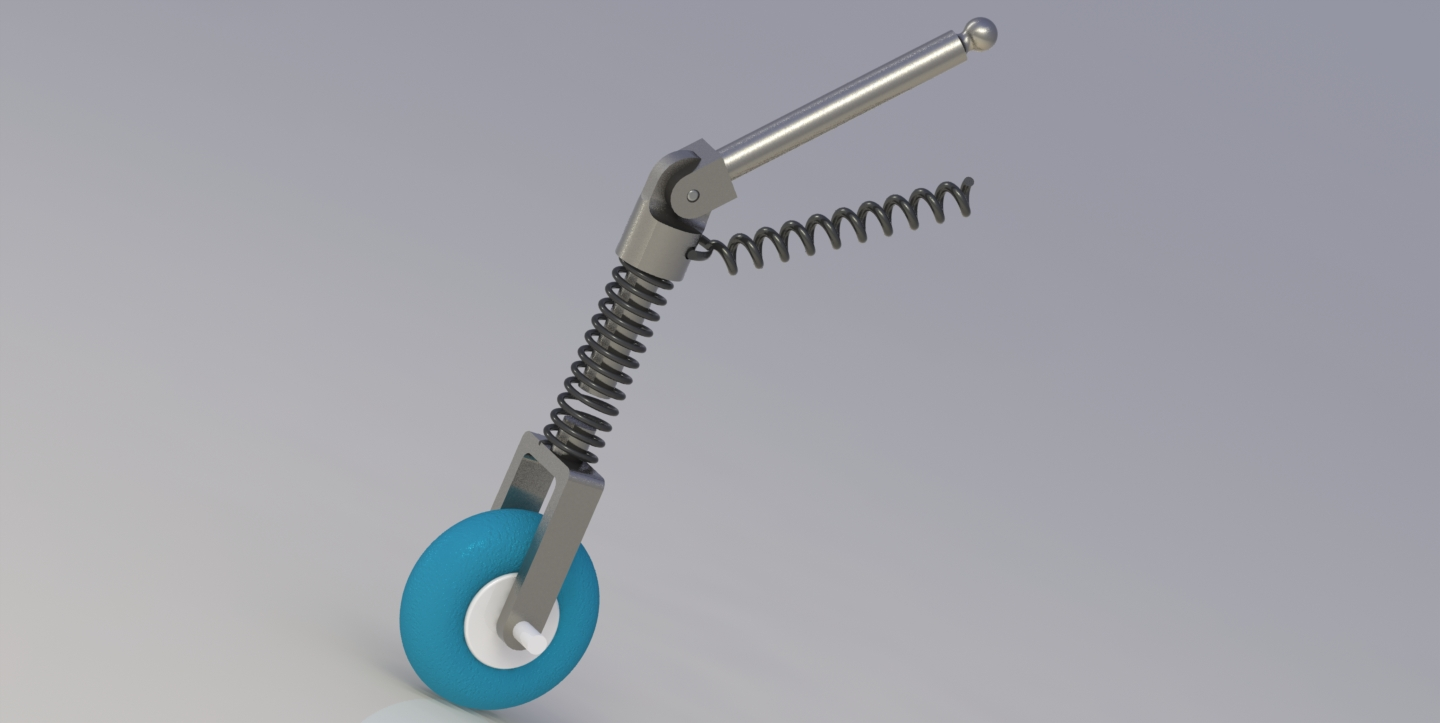
\includegraphics[width=0.8\textwidth]{chap2/EncoderWheel.JPG}}
  %\hspace{1in}
  \subfigure[部分工程图]{
    \label{fig:SensorSp:b} %% label for second subfigure
    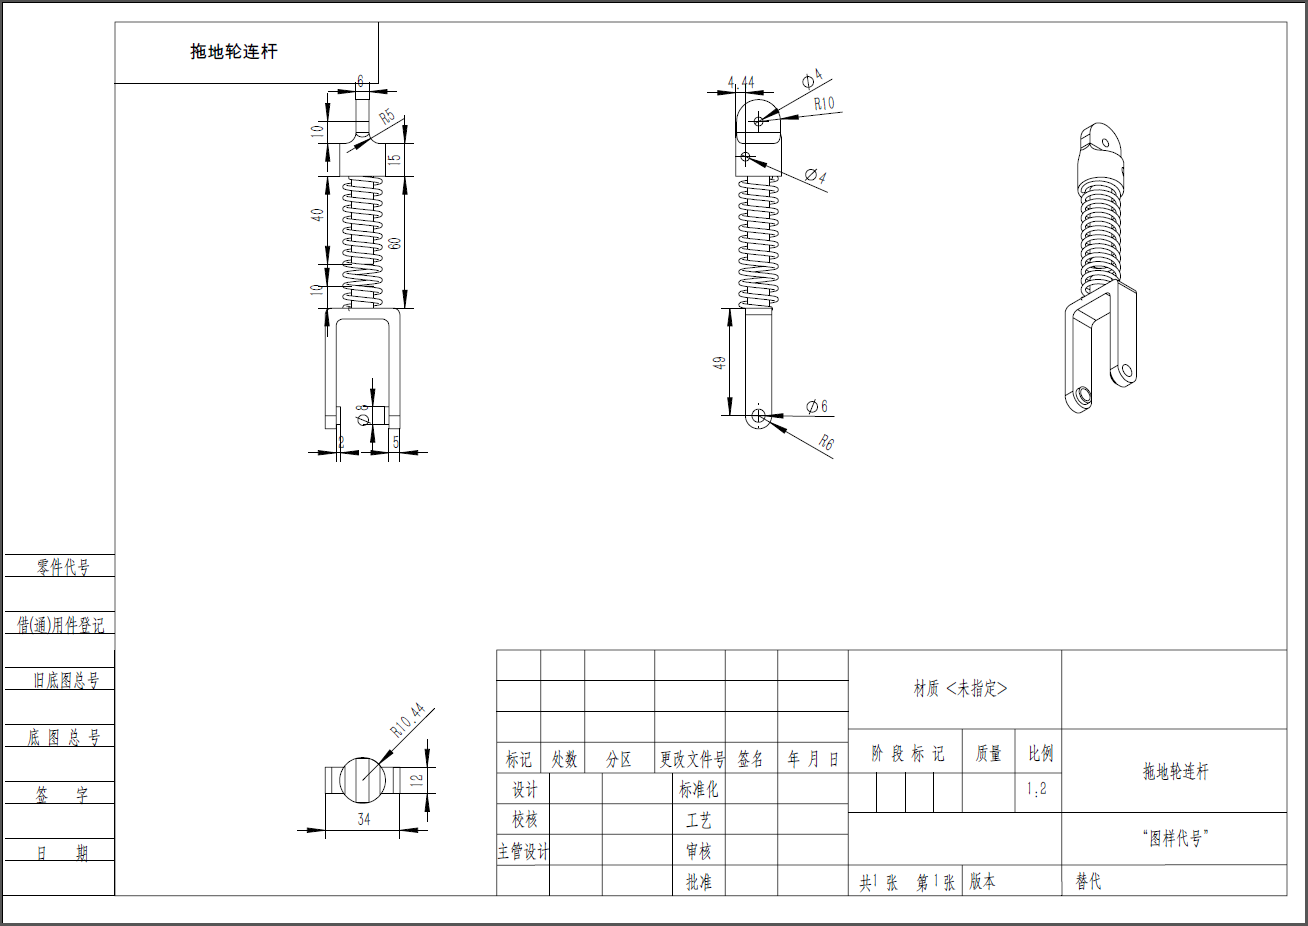
\includegraphics[width=0.8\textwidth]{chap2/encoderWheelPr.PNG}}
  \bicaption[fig.NewSensorSupport]{新设计的底盘编码轮三维立体图与工程图}{新设计的底盘编码轮三维立体图与工程图}{Fig}{The General Module of Independent Passive Wheel Encoder}
\end{figure}
\section{本章小结}
本章由已有的机器人设计出发,分析了以前设计的特点,并对设计中的不妥提出了疑问。再根据这些疑问出发,着手改进原来的设计方案。在本章中,详细的介绍了对于通用模块,传感器支架,模块连接机构,模块间传输单元机构和独立轮式编码单元的新的设计方案。通过新旧方案的对比,可以较为容易的 发现,新的设计方案克服了以前设计方案所存在的问题。
